\section{Quality Assurance}
\label{sec:fdsp-tpcelec-qa}

%%%%%%%%%%%%%%%%%%%%%%%%%%%%%%%%%%%
\subsection{Initial Design Validation}
\label{sec:fdsp-tpcelec-qa-initial}

As described above, four ASICs are being developed for the DUNE far detector single-phase TPC readout (LArASIC, COLDADC, COLDATA, and CRYO).  When a new prototype ASIC is produced, the first tests of ASIC functionality and performance are done by the groups responsible for the ASIC design.  These tests may use either packaged parts or dice mounted directly on a printed circuit board and wire bonded to the board.  The goal of these tests is to determine the extent to which the ASIC functions as intended, both at room temperature and at liquid nitrogen temperature.  For all chips these tests include exercising digital control logic and all modes of operation.  Tests of front-end ASICs include noise as a function of input capacitance, baseline recovery from large pulses, cross-talk, linearity, and dynamic range.  Tests of ADCs include effective noise and differential and integral non-linearity.  Tests of COLDATA and CRYO include verification of both the control and high speed data output links with cables at least as long at the longest cables needed in the DUNE far detectors (currently estimated to be 27 meters).

%%%%%%%%%%%%%%%%%%%%%%%%%%%%%%%%%%%
\subsection{Integrated Test Facilities}
\label{sec:fdsp-tpcelec-qa-facilities}

%%%%%%%%%%%%%%%%%%
\subsubsection{ProtoDUNE-SP}
\label{sec:fdsp-tpcelec-qa-facilities-pdune}

\dword{pdsp} is designed as a full slice of the \dword{spmod} as close as possible to the final 
DUNE \single components. It contains six full-size DUNE \dwords{apa} instrumented with \num{20} 
\dwords{femb} each for a total readout channel count of \num{15360} digitized sense wires. Critically, 
the wires on each \dword{apa} are read out via a full \dword{ce} readout system, including a \dword{ce} 
flange and \dword{wiec} with five \dwords{wib} and one \dword{ptc}. Each combined \dword{apa} and \dword{ce}
readout follows the grounding guidelines described in Section~\ref{G&S} to operate as a complete isolated
readout unit.

\dword{pdsp} took beam data in the CERN Neutrino Platform in 2018 and continued taking cosmic data 
into 2019. As described in Section~\ref{pdune results}, the live channel count (99.7\%) and average noise
levels on the collection and induction wires (ENC$<$600e$^-$ and 800$^-$, respectively) satisfy the DUNE
\single requirements described in Section~\ref{scope}. Several lessons learned from the production 
and testing of the \dword{ce} and the\dword{pdsp} 
beam data run will be incorporated into the next iteration of the system design for the \dword{spmod}.

Five of the six\dword{apa} were tested in the \dword{pdsp} Cold Box, which is described in
Section~\ref{sec:fdsp-tpc-elec-qa-facilities-atf}, prior to installation in the cryostat. These tests
were critical in identifying issues with \dword{ce} components after installation on the \dword{apa}. 
Therefore, a very similar set of Cold Box tests are being planned at SURF with the fully-instrumented
DUNE \single \dword{apa}.

The \dwords{apa} and the readout electronics will be different from the ones used in \dword{pdsp}; for 
this reason, plans are being made for re-opening the \dword{pdsp} cryostat and replacing three of the 
six \dwords{apa} with final DUNE prototypes that will also include the final versions of the 
\dwords{asic} and \dwords{femb}. A second period of data-taking with this new configuration of 
\dword{pdsp} is being planned for 2021-2022. This will also allow for another opportunity to check 
for interference between the readout of the \dword{apa} wires and either the \dword{pds} or other
cryogenic instrumentation.

%%%%%%%%%%%%%%%%%%
\subsubsection{Small Test TPC (ICEBERG)}
\label{sec:fdsp-tpcelec-qa-facilities-testtpc}

Fermilab is building an Integrated Cryostat and Electronics Built for Experimental Research Goals (ICEBERG). ICEBERG will be used for liquid Argon detector R\&D and DUNE Single Phase Cold Electronics (CE) prototypes, pre-production and production QA/QC. ICEBERG consists of a liquid Argon cryostat with cryogenic controls, 1280 channel DUNE Time Projection Chamber (TPC), with an Anode Plane Assembly and Field Cage, segmented CE Power distribution and Data Acquisition System. The TPC interface to the Cold Electronics is designed to adapt to future DUNE Front End Mother Boards. TPC has slots for inserting Photon Detectors.

The ICEBERG cryostat, shown in Figure~\ref{fig:ICEBERG-cryotee}, has been built by Ability Engineering to the design specification provided by Fermilab (Cryostat Design Specification). It is being installed at the Proton Assembly Building, Fermilab. The ASME B31.3 certified cryostat has an inner diameter of 152 cm and can hold about 35,000 liters of Liquid.

\begin{dunefigure}
  [ICEBERG cryostat and top plate Tee]
  {fig:ICEBERG-cryotee}
  {ICEBERG cryostat (left) and top plate Tee (right).}
  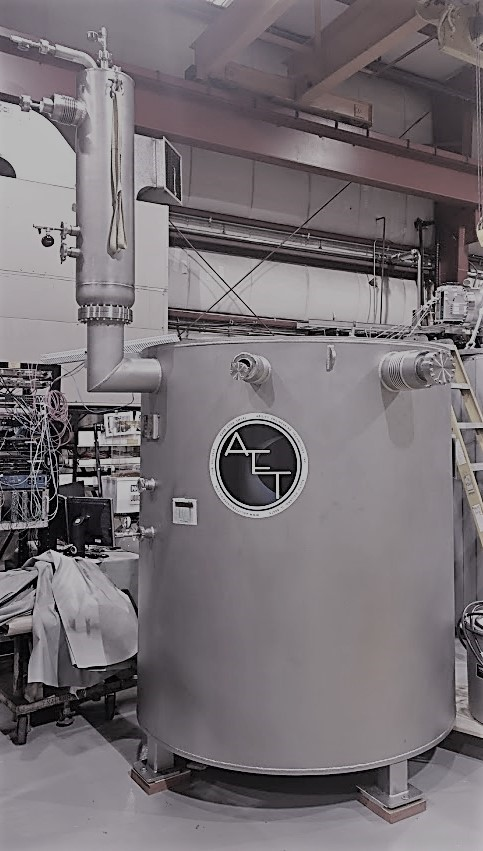
\includegraphics[width=0.3\linewidth]{sp-tpcelec-ICEBERG-cryostat.jpg}
  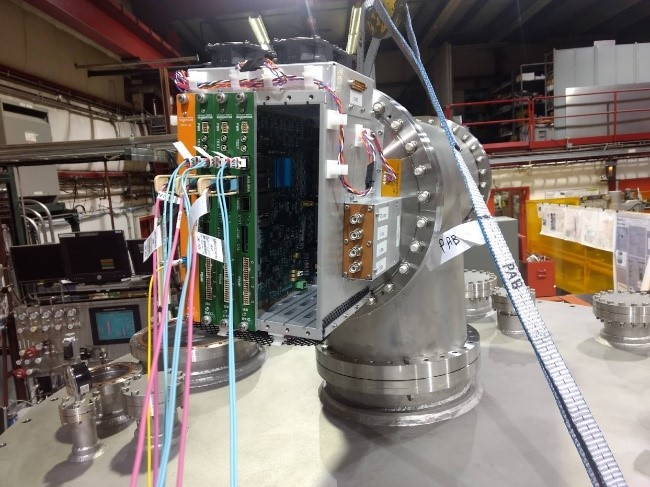
\includegraphics[width=0.6\linewidth]{sp-tpcelec-ICEBERG-Tee.jpg}
\end{dunefigure}

A detector of about 125 cm x 125 cm x 60 cm can fit inside the cryostat. The power and signal cables for the detector are routed through a Tee installed on the center port. 14 additional ports are available for different utilities including HV feed through, purity monitor, cryogenic controls and visual inspection. Condenser, liquid Argon fill and vacuum ports are at the side of the cryostat, providing easy access to the detector.

On the top of the cryostat a Tee is installed for holding the Cold Electronics Warm Interface Board, Power and Signal Cables, Photon Detector cables.

The Time Projection Chamber (TPC) has a 1280 Anode Plane Assembly (APA) (see Figure~\ref{fig:ICEBERG-tpcdaq}), Field Cage and Two Cathode planes. The APA has been built following the same design as for ProtoDUNE.

\begin{dunefigure}
  [ICEBERG TPC and DAQ rack]
  {fig:ICEBERG-tpcdaq}
  {ICEBERG TPC (left) and DAQ rack (right).}
  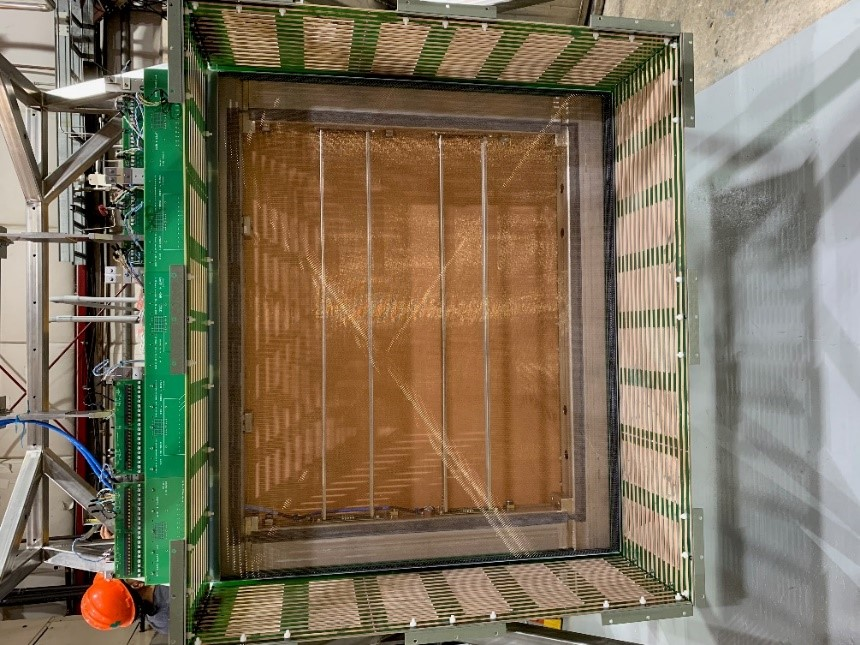
\includegraphics[angle=270,width=0.45\linewidth]{sp-tpcelec-ICEBERG-TPC.jpg}
  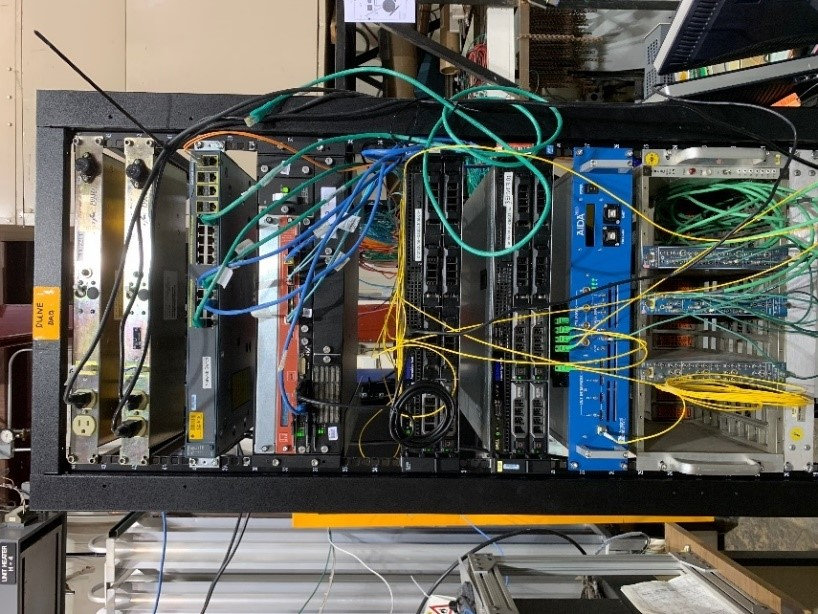
\includegraphics[angle=270,width=0.4\linewidth]{sp-tpcelec-ICEBERG-DAQ.jpg}
\end{dunefigure}

The Field cage for the TPC is construction using printed circuit boards and is designed to provide 25 cm of drift space on either sides of APA. The cathode plane is made of a PC board coated with copper and will be powered with -15 KV DC power. There is a 1 Giga Ohm resistance between each field cage strips making a gradient field going from cathode plane of -15 KV to -1 KV near the APA. The two sides of the Field cages are terminated to the APA ground by 156 mega Ohms resistance. 

The DUNE Cold Electronics is interfaced with the APA using the printed circuit board on the top of the APA.

The ICEBERG power system that would power the detector, electronics, DAQ and cryogenics controls has been designed with an extreme care to isolate the detector and building grounds. A new 480 Volts transformer has been installed at the Proton Assembly Building to provide detector power for the TPC and the Cold Electronics. The impedance is continuously monitored by a ZMON rack. 

The distribution panel, which is at detector ground provides 208 and 120 volts power for the COLD Electronics Rack, which provides power to both the Cold Electronics and TPC in the cryostat through the Warm Interface Board and Power Points located in the Tee (see Figure~\ref{fig:ICEBERG-cryotee}). The MPOD in CE Power Rack provides -665, -370, 0 and 820 Volts to Grid, U, V and X planes respectively. It also provides -15 k Volts to the cathode plane. The Wiener PL506 provides 18, 48, 12 and -12 volts to the Power and Timing Card (PTC) located in the Tee at the top of the cryostat. These voltages are distributed to FEMB through the Warm Interface Board through the back plane of the crate.

The Data Acquisition (DAQ) System for the ICEBERG consists of several subsystem currently being utilized at the ProtoDUNE at CERN.

The system is modular and could be upgraded to follow the overall DUNE DAQ development. The core of the DAQ system consists of two Scientific LINUX CPUs which communicates over 10 Gbps optical fiber links to Cluster on Board (COB). COB collects raw data from the Cold Electronics Warm Interface Board (WIB) over fiber and packages them for analysis by artDAQ running of the UNIX CPU. A pair of scintillators located at the top and bottom of the cryostat generates a cosmic trigger for the DAQ  using a Trigger Logic Unit (TLU).

The ICEBERG will be primarily used for the development of the DUNE Cold Electronics. The initial system to establish a baseline for future comparison and development closely resembles the DUNE CE installed in ProtoDUNE at CERN. It consists of a 128 channels Front-End Mother Board, which is enclosed in a RF Box and connected with a Power and Signal cables to Warm Interface Board. The Warm Interface Board is located in a crate inside the Tee (Fig 1 (b)) and is powered using a Power and Timing Card.

In the 1st run of the cryostat we will establish the baseline performance of the DUNE Cold Electronics. Studies will be carried out to understand noise in the electronics and measures to reduce them. A new FEMB is under design by the collaboration. All the FEMB will be replaced with new electronics and studies will be performed to verify that the new design meets the DUNE requirements. The facility could be utilized for QA/QC if the electronics before installing them in the Far Detector.

%%%%%%%%%%%%%%%%%%
\subsubsection{Additional Test Facilities}
\label{sec:fdsp-tpcelec-qa-facilities-additional}

For \dword{ce} development, testing single prototypes at both room and cryogenic temperature is the first 
step, as many problems can be identified quickly without a full or partial TPC wire readout. A test dewar 
design developed by Michigan State University, referred to as the Cryogenic Test System (\dword{cts}), allows for
testing of the \dwords{femb} and \dwords{asic} at both room temperature and submerged in LN$_2$. Several
\dword{cts} were deployed at BNL for the \dword{pdsp} production \dword{femb} QC and SBND \dword{asic} QC. Several
others have already been deployed as Fermilab and other institutions to test further prototype \dword{femb}.
The \dword{cts} cooling process avoids the condensation of water from air that can otherwise interfere with the 
tests or damage the test equipment; two \dword{cts} units in operation at BNL are shown in Figure~\ref{fig:CTS}.

\begin{dunefigure}
[The Cryogenic Test System (\dword{cts})]
{fig:CTS}
{Cryogenic Test System: an insulated box is mounted on top of a commercial LN$_2$ dewar.  Simple controls allow the box to be purged with nitrogen gas and LN$_2$ to be moved from the dewar to the box and back to the dewar.}
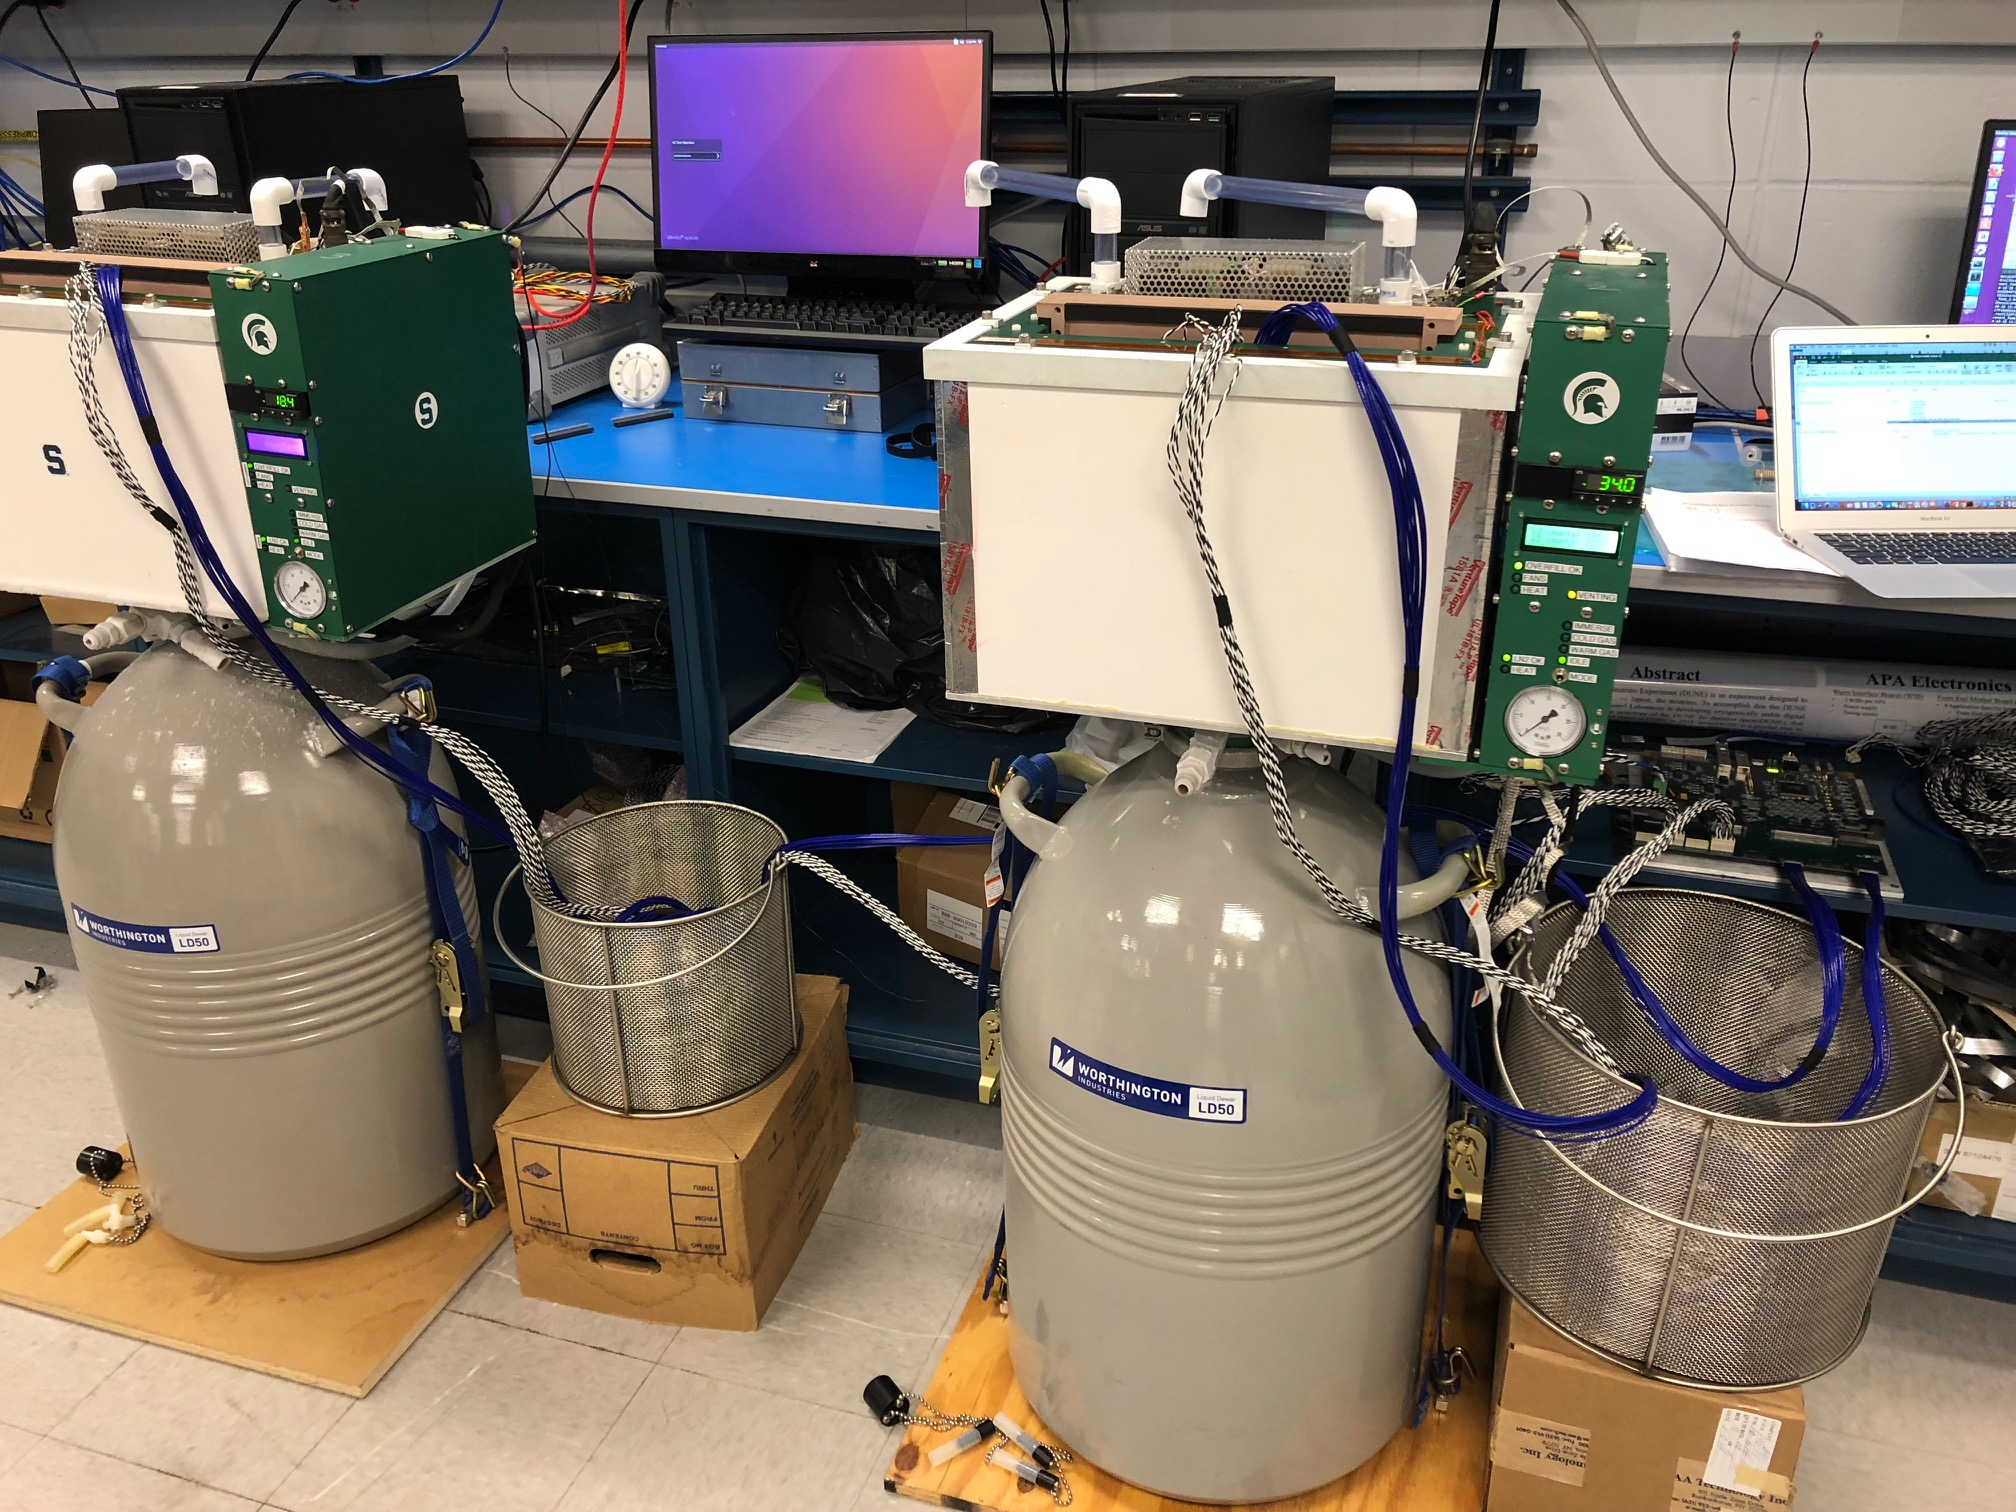
\includegraphics[width=0.4\linewidth]{sp-tpcelec-CTS2.jpeg}
\end{dunefigure}

Additionally, a quick access test stand with the \dword{femb} connected to an \dword{apa} inside a shielded 
environment that is in the same location as the \dword{femb} and \dword{asic} development is invaluable 
for rapid progress.  Two such facilities are available to DUNE: the ``ICEBERG'' small TPC at \fnal and the 
\num{40}\,\% \dword{apa} test stand at BNL. ICEBERG will be described in Section~\ref{iceberg-sux}.

The \num{40}\,\% \dword{apa} at BNL is a \SI{2.8}{m}~$\times$~\SI{1.0}{m} three-plane \dword{apa} with two 
layers of \num{576} wrapped ($U$ and $V$) wires and one layer of \num{448} straight ($X$) wires. It is read 
out by up to eight \dwords{femb} with the full \SI{7}{m} \dword{pdsp} length data and \dword{lv} power cables, 
four on the top and four on the bottom. The readout uses the full \dword{ce} system, with \dword{ce} flange 
and \dword{wiec}, as shown in Figure~\ref{fig:tpcelec_40apa}. Detailed integration tests of the \dword{pdsp}
\dword{ce} readout performance while following the DUNE grounding and shielding guidelines were done at the 
\num{40}\,\% \dword{apa}.

\begin{dunefigure}
[One side of the \num{40}\,\% \dword{apa} with four \dwords{femb} and the full \dword{ce} \fdth and flange.]
{fig:tpcelec_40apa}
{Left: one side of the \num{40}\,\% \dword{apa} with four \dwords{femb}.  Right: the full \dword{ce} \fdth and flange.}
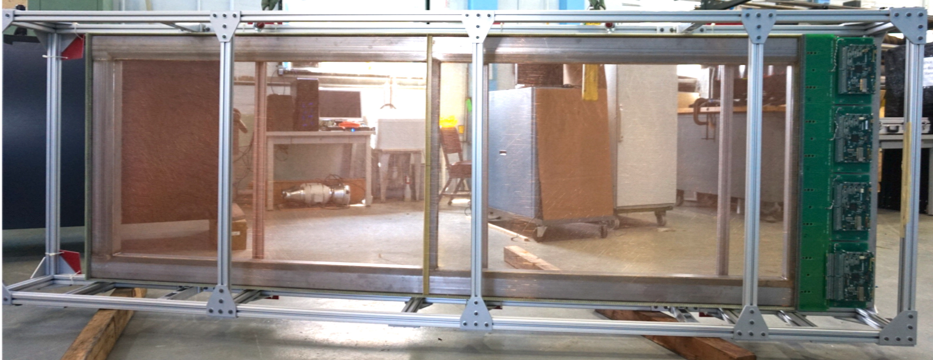
\includegraphics[width=0.72\linewidth]{sp-tpcelec-40-apa.png}
\hspace{3mm}
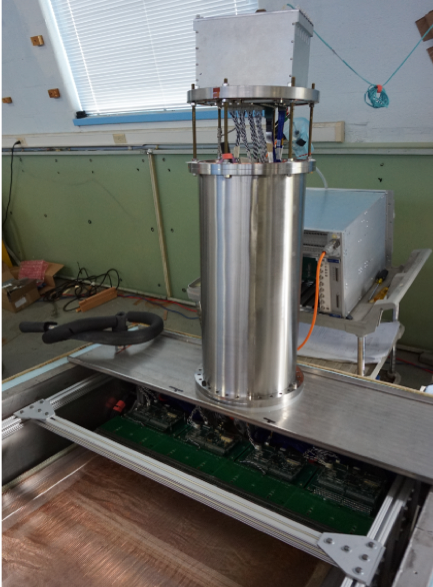
\includegraphics[width=0.2\linewidth]{sp-tpcelec-40-apa-ft.png}
\end{dunefigure}

%Additional input capacitance (equivalent to longer wire length) have been added to a subset of channels to project the \dword{enc} performance from the 40\% \dword{apa} teststand to the \dword{pdsp} and SBND detectors. The results from the \num{40}\,\% \dword{apa} indicate that, if the new \dword{adc} performs as expected, the full \dword{ce} system as installed on the test  stand at BNL will have a noise level in \lar around \num{500}\,e$^-$ and \num{600}\,e$^-$ for the collection and induction plane channels, respectively, in line with the CERN cold box tests described in Section~\ref{sec:fdsp-tpc-elec-qa-facilities-coldbox}.

%\begin{figure}
%    \centering
%    \includegraphics[width=0.9\linewidth]{tpcelec-40-apa-result.png}
%    \caption{\dword{enc} (in electrons) as a function of input capacitance (equivalent to input wire length) measured on the 40\% \dword{apa}. The \dword{enc} projections are based on the input wire length of the SBND and \dword{pdsp} detectors.}
%    \label{fig:tpcelec_40\dword{apa}_results}
%\end{figure}

Additionally, a Cold Box at CERN used in electronics tests for \dword{pdsp} is available for electronics testing 
in cold nitrogen gas. The advantage of the Cold Box is that it can cycle one full-size \dword{apa} with the full 
set of \num{20} \dword{femb} through gaseous nitrogen temperatures around \SI{150}{K} to validate the \dword{apa} 
performance as a complete \dword{ce} readout unit, as opposed to the 40\% APA and ICEBERG each of which have smaller
\dword{apa} footprints with fewer wires. The Cold Box is designed to be a Faraday cage, using the same grounding 
and shielding scheme that is implemented for the DUNE \single cryostat. It is read out by a complete \dword{ce} 
system for a single \dword{apa}, including a \dword{ce} flange and fully-loaded 
\dword{wiec} with five \dwords{wib} and one \dword{ptc}. Preliminary results from the \dword{pdsp} Cold Box testing 
for the second \dword{apa} installed at CERN are shown in Section~\ref{protodune-sux}.

%%%%%%%%%%%%%%%%%%%%%%%%%%%%%%%%%%%
\subsection{Reliability Studies}
\label{sec:fdsp-tpcelec-qa-reliability}

The TPC cold electronics system of the DUNE single phase far detector has to meet stringent requirements, such as low ($<<$ 1\%) failure rate of components installed on detector, inside the cryostat, without easy access during 20+ years of detector operation. Reliability of all the components must be incorporated in the design and a dedicated analysis of all the possible failure mechanisms is required before finalizing the design of all ASICs, printed circuit boards, cables, connectors, and their supports, all of which are housed inside the DUNE far detector cryostat. 

There are a few HEP detectors that have been operated without intervention for a prolonged period of time, with limited losses of readout channels, and in extreme conditions like those of the DUNE cryostats:
\begin{itemize}
	\item NA48/NA64 liquid Krypton (LKr) calorimeter has 13,212 channels of JFET preamplifiers installed on detector. It has been kept at LKr temperature since 1998. The failure rate is $<$ 0.2\% for 20 years of operation so far.
	\item ATLAS liquid Argon (LAr) accordion EM Barrel (EMB) calorimeter has $\sim$110,000 readout signal channels, with up to seven connections and different circuit boards populated with resistor and diodes inside cryostat. The EMB calorimeter has been cold since 2004, for 14 years of operation.  So far the failure rate of readout channels is $\sim$0.02\%.
	\item ATLAS liquid Argon Hadronic Endcap Calorimeter (HEC) has $\sim$5,600 readout channels through $\sim$35,000 cold preamplifier channels designed in GaAs technology on preamplifier and summing boards (PSB). The HEC cold electronics has been in cold operation since 2004, with $\sim$0.37\% failure rate during 14 years of operation. 
\end{itemize}
In addition, FERMI/GLAST is an example of a joint project between NASA and HEP groups that had a minimum mission requirement of five years and is on its way to achieving a stretch goal of ten years of operations in space. As the requirements can be rather different, it is important to examine and understand the various strategies for a space flight project compared to those of DUNE. Specifically launch "Shake and Bake" tests, redundancy requirements on critical infrastructure, and extensive test to failure, etc., may be inapplicable.

A preliminary list of reliability topics to be studied for the TPC electronics operated in LAr environment are:
\begin{itemize}
	\item The custom ASICs proposed for use in DUNE (BNL FE ASIC + joint LBNL-FNAL-BNL ADC + COLDATA ASIC, or the SLAC CRYO ASIC) incorporate design rules aimed at minimizing the hot carrier effect\cite{Li:2013ieee}\cite{Hoff:2015hax}, which is recognized as the main failure mechanism for integrated circuits operating at LAr temperature.
	\item For COTS components, accelerated lifetime testing, a standard test methodology used by the semiconductor industry, shall be devised to verify the expected lifetimes for operation in cryogenic temperature. A COTS ADC has undergone this procedure, to be qualified as a solution for the SBND experiment\cite{Chen:2018zic}.
	\item Print circuit board assemblies designed and fabricated to survive repeated immersions in LN$_2$.
	\item Capacitors operating voltage with sufficient margin, e.g. V$_{OP}<$ WVDC/2.
	\item Connectors and cables, usually major sources of detector channel failures, impose a testing challenge.
	\item A formal QA process for all TPC electronics components to be installed inside the cryostat.
\end{itemize}
The DUNE CE consortium has formed a working group tasked with studying reliability issues of these CE components and is preparing recommendations for the choice of ASICs, the design of printed circuit boards, and testing. This working group will review the segmentation of the cold electronics to understand which failures are going to have the largest impact on data taking; revisit recommendations for the ASIC design, beyond those aimed at minimizing the hot carrier effect; revisit the industry and NASA standards for the design and fabrication of printed circuit boards, connectors, and cables, and make recommendations for the QA/QC procedures to be adopted during the fabrication of the cold electronics components. And in the review of the system aspects, to understand where it is desirable, necessary, and feasible to implement redundancy in the system, to minimize data losses due to single component failures. Later this working group will develop the QC program for the CE detector components, based upon experience from the ProtoDUNE-SP project.
